% This is appa.tex
%
% This file is for appendices.  If you don't have any appendices, delete
% the percent sign from the beginning of the next line.
%\endinput

\clearpage
\appendix
\section{Appendix: Figures and Tables}

\begin{figure}[h!]
    \centering
    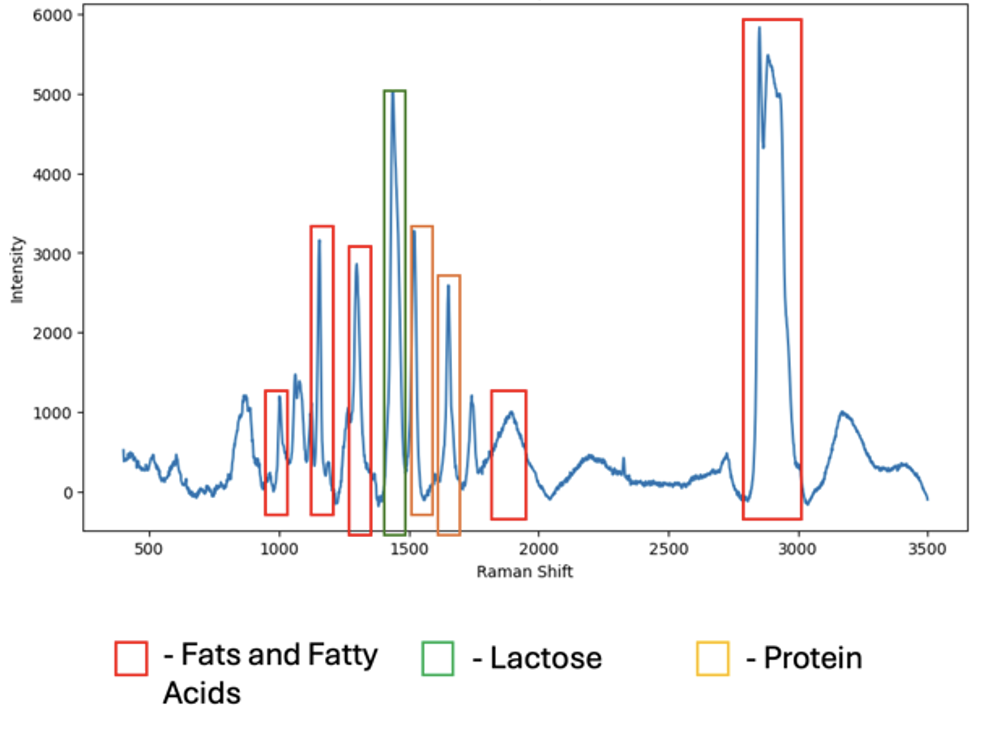
\includegraphics[width=0.5\linewidth]{Figures/Screenshot 2025-07-16 at 2.26.41 PM.png}
    \caption{Characterization of Raman Peaks for the Control Sample}
    \label{fig:ram}
\end{figure}

\begin{table}[h!]
\centering
\begin{tabular}{|l|c|l|}
\hline
\textbf{Functional Groups} & \textbf{Raman Band (cm\textsuperscript{-1})} & \textbf{Component} \\
\hline
Aromatic C--C & 1016 & Fat \\
CH\textsubscript{2} twist, Ester & 1279, 1315 & Fat \\
CH\textsubscript{2} bending & 1416, 1759 & Fat, Lactose \\
Amide I & 1566 & Proteins \\
Amide II & 1670 & Proteins \\
CH stretch & 2865, 2902 & Fatty Acids \\
\hline
\end{tabular}
\caption{Raman spectral bands of various functional groups in milk components}
\label{tab:raman_bands}
\end{table}


\begin{figure}[h!]
    \centering
    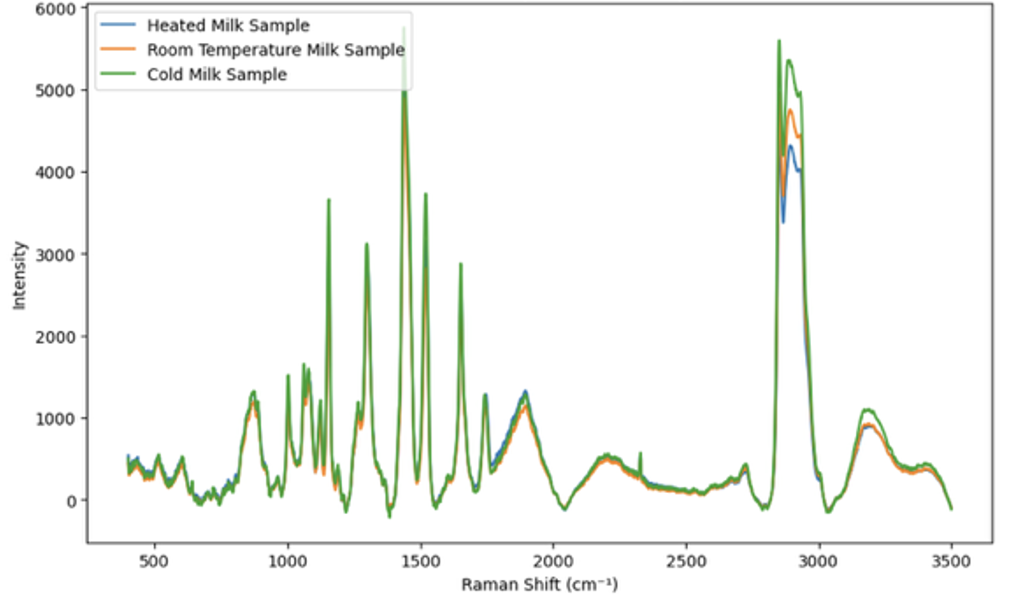
\includegraphics[width=0.5\linewidth]{Figures/Screenshot 2025-07-16 at 2.27.09 PM.png}
    \caption{Variation in Raman Spectra of Control Sample with Temperature}
    \label{fig:temp}
\end{figure}

\begin{figure}[h!]
    \centering
    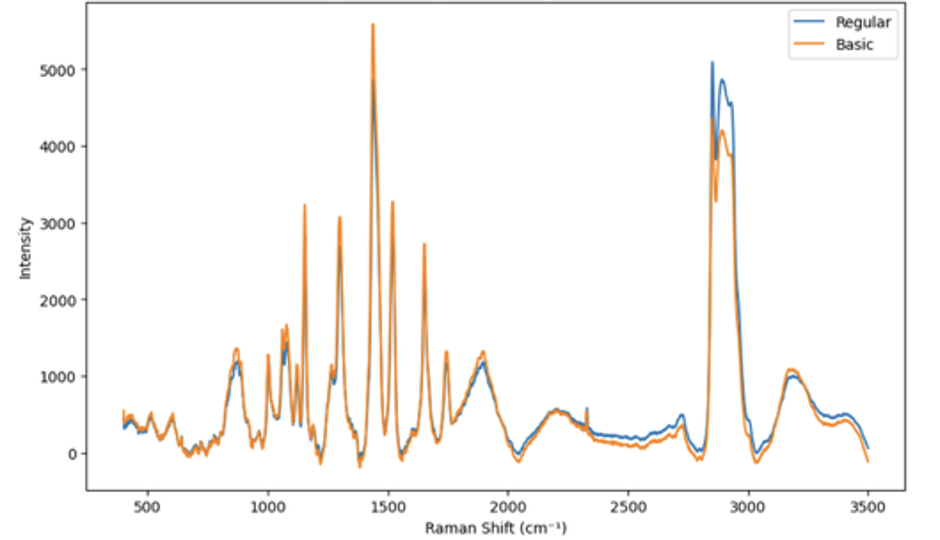
\includegraphics[width=0.5\linewidth]{Figures/Screenshot 2025-07-16 at 2.27.24 PM.png}
    \caption{Variation in Raman Spectra of Control Sample with pH}
    \label{fig:confusion}
\end{figure}

\begin{figure}
    \centering
    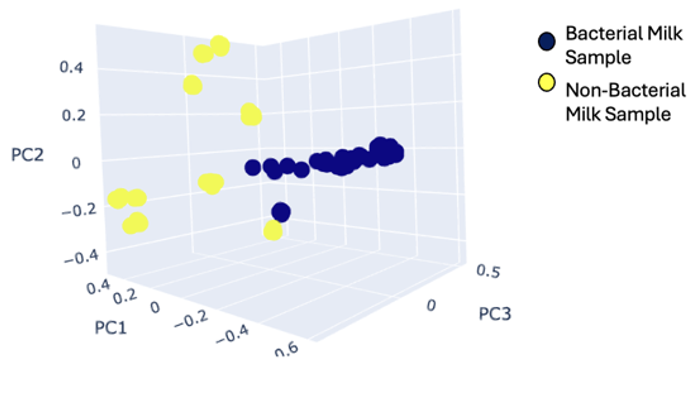
\includegraphics[width=0.5\linewidth]{Figures/Screenshot 2025-07-16 at 2.27.37 PM.png}
    \caption{PCA Analysis of Bacterial and Non-bacterial samples}
    \label{fig:bac}
\end{figure}

\begin{figure}
    \centering
    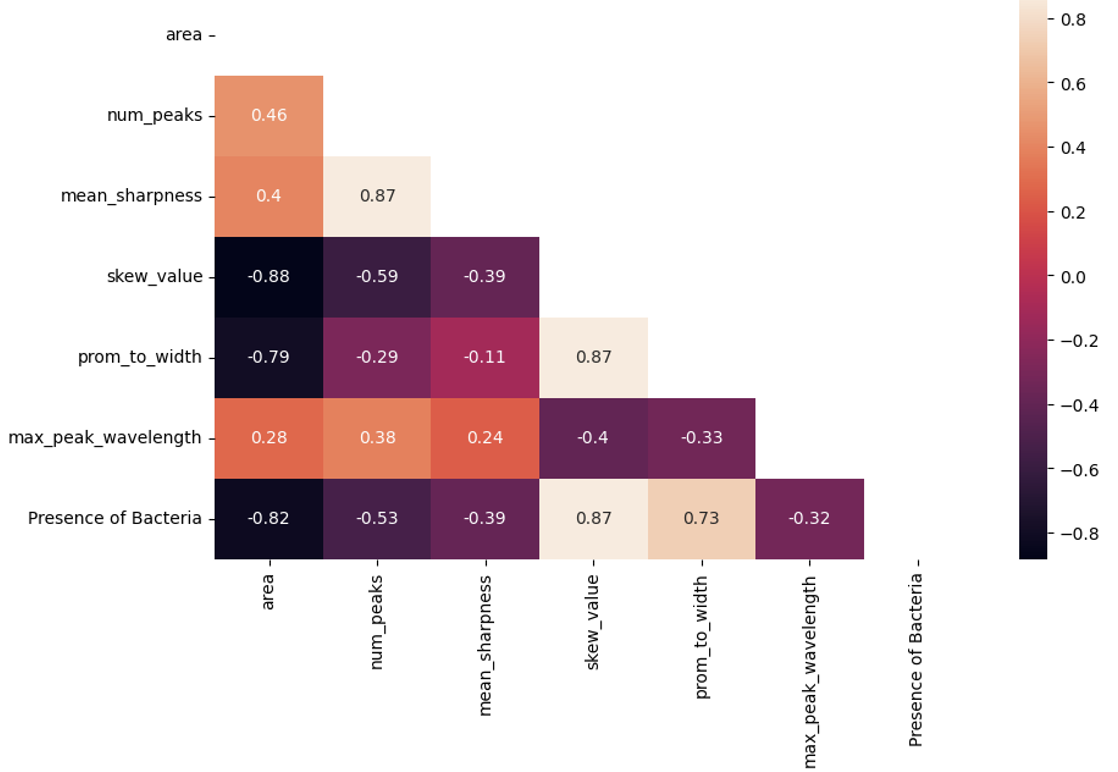
\includegraphics[width=0.5\linewidth]{Figures/Screenshot 2025-07-16 at 2.27.59 PM.png}
    \caption{Correlation Analysis of Feature Extracted Variables}
    \label{fig:corr}
\end{figure}

\begin{figure}
    \centering
    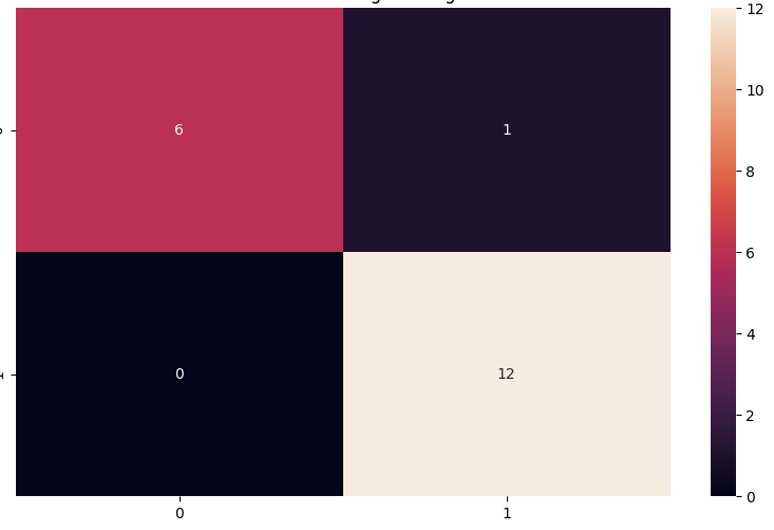
\includegraphics[width=0.5\linewidth]{Figures/Screenshot 2025-07-16 at 2.28.32 PM.png}
    \caption{Confusion Matrix for Logistic Regression, Support Vector Machines and Naive Bayes Classifier}
    \label{fig:cm}
\end{figure}

\begin{figure}
    \centering
    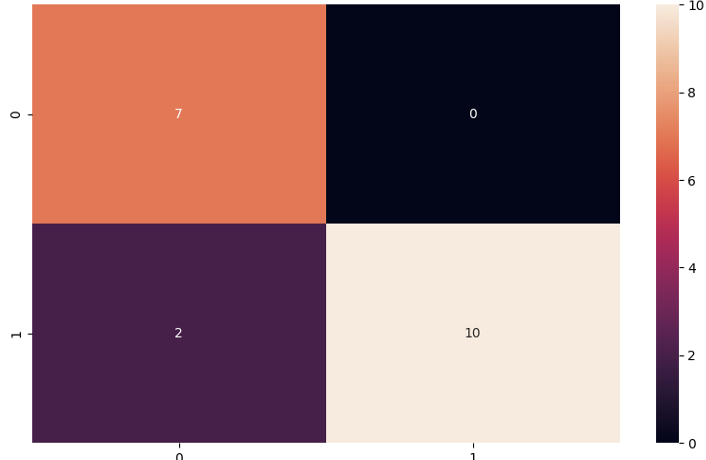
\includegraphics[width=0.5\linewidth]{Figures/Screenshot 2025-07-16 at 2.28.53 PM.png}
    \caption{Confusion Matrix for Gaussian Process Classifiers}
    \label{fig:cm2}
\end{figure}
